% Chapter 2

\chapter{Introduction} % Chapter title

\label{ch:examples} % For referencing the chapter elsewhere, use \autoref{ch:examples} 

%----------------------------------------------------------------------------------------

Probability has compelled beyond all alternatives as a representation of knowledge in domains rife with uncertainty; and probabilstic inference correspondingly so as a method for reasoning.
The success story is only partially written however; while Bayes' Rule states how we should update our beliefs in hypotheses conditioned on evidence, it tells us only declaratively, and leaves us with no indication of such.
In a sense we have been provided with the logic.

The majority of current 
hese models explain how learners select among competing
hypotheses; for the most part, they do not attempt to explain how learners construct
hypotheses in the first place.
Hypothesis. However, efficiently sampling
hypotheses is not the same as constructing them.

Perhaps.
However, with only the minimal constraints of simplicity,
grammaticality, and previously productive templates, changes to hypotheses generated by
random variation seems at best inefficient. More importantly, our minds seem to have
access to rich sources of information that could better constrain the process of hypothesis generation and that current approaches do not exploit.

Buildon upon recently interpretations of inference in computational terms, I am to incorporate conditions constructively into generative models.
That is, given a generative model manifested as a stochastic {\em prior program} $P$, and a conditioning predicate $C$ we wish to construct a new program $P^*$ which samples only values which adhere to our constraints and remains.
The approach here attempts to concretise many of the concepts outlined in \citep{SHULTZ}
, and perhaps suprisingly, we draw more from the fields of program semantics.

The feasibility of this aim is vulnerable; if it were possible to
Consider the ease with which you can compose a paragraph that rhymes, generate a polynomial expression, draw a graph without cycles.
From a probabilstic inference perspective, each of these examples can be considered a generative model compared with a condition, and our ability to perform such tasks is probabilstic inference.

A further appeal of such as approach is its potential to bridge between discriminative and generative approaches
Discriminative models may detect broad level characteristics of a scene, while generative use these as constraints.

First we will summarise \spacedlowsmallcaps{query}, a computational theory of probabilstic inference.
The propose then outline many approaches
Three approaches to implementing CONSTRAIN are outlined

%----------------------------------------------------------------------------------------

\subsection{Query}

QUERY is a formalism of probabilstic inference stated explicitly in computational terms; our explanation is stated in terms of models of computatins.
Developed first as a primitive function in the probabilstic programming language Church \citep{CHURCH}, elaborated on in \citep{VIKASH}.

LAMBDA CALCULUS INTERPRETATION
In \citep{FREER:2012}, query is formulated as a probalistic turing machine (PTM), which takes two inputs, a prior program $P$ and a conditioning predicate $C$.
Both $P$ and $C$ are themselves encodingings of PTMs that take no input.
QUERY generates a sample from P.
Then, if $X$ is satisfied, then this sample is outputted, otherwise the process is repeated.

\begin{verbatim}
(define (query exp pred)
  (let ((val (eval exp))
    (if (pred val)
        val
        (query exp pred)))))
\end{verbatim}

\subsection{Constrain}
The semantics of \spacedlowsmallcaps{constrain} can be readily understood in terms of QUERY.
If we take the above lamba-calculus definition of query, as a function, CONSTRAIN can eb viewed simply as query with all its arguments partially evaluated.

\begin{verbatim}
(define (constrain exp pred)
  (fn [] ))
\end{verbatim}

Simply put, query returns a sample given a model and condition, while constrain given the same input returns a function of no arguments which calls query.

The difference can be seen as the difference from sampling $P(x\vert C)$ or constructing a new prior $P^*(x)$.

This alone is not a large step, what is important is to retain that condition $C$

% Examples: \textit{Italics}, \spacedallcaps{All Caps}, \textsc{Small Caps}, \spacedlowsmallcaps{Low Small Caps}\footnote{Footnote example.}.

%------------------------------------------------

\subsection{Distribution Conserving}
Distribution preserving or not
How to deal with constraints

\graffito{Note: The content of this chapter is just some dummy text.}

\chapter{Constrained Generative Models}
There are a number of ways to explore this problems, varying principally in domain specificity, declarativeness of specification.

\section{Transform naive generative model}
Transformational Programming is a prominent method used in automated program development.
A formal, declarative specifciation of a program is {\em refined} into a complete program by applying a sequence of correctness-preserving transformations.
We can appropriate this framework for our purposes; transform a naive generative into a semantically equivalent (and hence distribtuion equivalent) program.

From a stochasic program $P$ and constraint $C$, we construct a new program $R_P^C$ with rejection sampling semantics.
$R_P^C$ executes $P$ to sample from its prior and returns the sample $C$ is satisfied, otherwise a further attempt is made.
Formally we can describe $R_P^C$ as a partially-evaluated higher order function, in lisp notation:

\graffito{Partial evaluation of a program means to take some subset of its arguments, and compile a new program with this subset fixed (under closure) and no longer arguments.}
\begin{verbatim}
(defn R [P C]
  (let [sample (P)]
  (if (true? (C sample))
      sample
      (R P C))))
\end{verbatim}

Our next objective is to perform a series of transformations to improve the efficiency $R_P^C$.
By constraining this set of transformations to be semantic preserving; that is any new program.

\subsection{Domain specificity}

\subsection{Domain specificity}

\section{Error correcting evaluation}
Dependencies on domain specific knowledge is problematic.
Representing 
The alternative seems even more implausible; how can one generate only convex polygons without any understanding of  convexity, and more generally geometry.

The approach described here takes a middle ground to circumvent an ostensible requirement for doman specific knowledge.
First, by treating our conditions as computable functions, predicates themselves contain a wealth of information, which may be sufficient.
The idea is to not treat these predicates as black boxes, but instead to analyse their structure.
Second structured objects can be decomposed into parts, and unsatisfiability can be {\em blamed} on subcomponenets.
We can fix a 
In other words, neither our predicates nor objects upon which predicates are applied are monolithic, impenetrable black boxes

\subsection{Program Transparency}
TODO EXPLAIN PROGRAM TRANSPARENCY BOTH INFORMALLY AND ATTEMPT A FORMAL DEFINITION

\subsection{Blame attribution}
The approach outlined here has for the moment at least been namde error correcting evaluation.
This is because the process is derived from program evaluation, or interpretation.
The general goal is to evaluate our condition $C$ find the causes of unsatisfiability, that is, attribute blame for our to some portion of the code.
Then, we seek to figure out alternative words (execution traces), that would cause this unsatisfiability to become satisfied.

\subsection{Unification: Attribution blame to the generative model}
The

\subsection*{Filter generative model}.  From $D$ derive a {\em filter function} $f$ which transforms a sample from a naive model to one which satisfies $D$.
That is $f:O \rightarrow O^*$, where $ \bigwedge\limits_{i} d_i(o^*) = 1$.
Examples of $f$ could be convex hull algorithms, cycle removing, or variable separation.
Although in both this and the first approach we seek a sample which satisfies $D$, there are important differences.
Here we do not reformulate the problem in optimisation terms, and seek a transform which will directly result in our constraints being satisfied.
Clearly, as exemplified 

Questions
What if all the constraints can't be satisifed, do we want partial satisfaction, do we want to know?

\chapter{Case study}
Either
1. Polygon example
2. 
\section{Optimise initial sample}.  Preliminary evidence has suggested that choosing a good initial sample has convergence advantanges.
Both inference and search methods begin with an initial sample or configuration, sampled from the prior distribution or chosen arbitrarily.
The idea here is to optimise this initial sample such that it adheres to our set of constraints.
Formally our objective in search is given some configuration space $X$, and a cost function $f:X \rightarrow \mathbb{R}$, our objective is to find $argmin_x f$.
In inference terms we would like to sample from a posterior distribution $P(X \vert Y)$.

Additionally, given a set of declarative constraints $D$ where $d \in D:X \rightarrow \{0,1\}$, we wish to find an initial sample or configuration $o_0 \in O$, which minimises some function $g(d_1(o_0),..,d_n(o_0))$.  $g$ is required to balance multiple constraints and a simple example could be $g(p_1,.,p_n) = \sum_i{1 - p_i}$.


Domain general.
Unsure how useful this? Will need to test
If I just want a new gen model, not doign inference, I could optimise every sample, but then my new distribution would be dependent on my optimisation dynamics.
Choice is g is rather arbitrary
How to do the optiisation?


%------------------------------------------------

\subsection{Autem Timeam}

\lipsum[6]

%----------------------------------------------------------------------------------------

\section{Another Section in This Chapter}

\lipsum[7]

Sia ma sine svedese americas. Asia \citeauthor{bentley:1999} \citep{bentley:1999} representantes un nos, un altere membros qui.\footnote{De web nostre historia angloromanic.} Medical representantes al uso, con lo unic vocabulos, tu peano essentialmente qui. Lo malo laborava anteriormente uso.

\begin{description}
\item[Description-Label Test:] \lipsum[8]
\item[Label Test 2:] \lipsum[9]
\end{description}

\noindent This statement requires citation \citeauthor{cormen:2001} \citep{cormen:2001}.

%------------------------------------------------

\subsection{Personas Initialmente}

\lipsum[10]

\subsubsection{A Subsubsection}
\lipsum[11]

\paragraph{A Paragraph Example} \lipsum[12]

\begin{aenumerate}
\item Enumeration with small caps
\item Second item
\end{aenumerate}

\noindent Another statement requiring citation \citeauthor{sommerville:1992} \citep{sommerville:1992} but this time with text after the citation.

\begin{table}
\myfloatalign
\begin{tabularx}{\textwidth}{Xll} \toprule
\tableheadline{labitur bonorum pri no} & \tableheadline{que vista}
& \tableheadline{human} \\ \midrule
fastidii ea ius & germano &  demonstratea \\
suscipit instructior & titulo & personas \\
\midrule
quaestio philosophia & facto & demonstrated \citeauthor{knuth:1976} \\
\bottomrule
\end{tabularx}
\caption[Autem timeam deleniti usu id]{Autem timeam deleniti usu id. \citeauthor{knuth:1976}}  
\label{tab:example}
\end{table}

\enlargethispage{2cm}

%------------------------------------------------

\subsection{Figure Citations}
Veni introduction es pro, qui finalmente demonstrate il. E tamben anglese programma uno. Sed le debitas demonstrate. Non russo existe o, facite linguistic registrate se nos. Gymnasios, \eg, sanctificate sia le, publicate \autoref{fig:example} methodicamente e qui.

Lo sed apprende instruite. Que altere responder su, pan ma, \ie, signo studio. \autoref{fig:example-b} Instruite preparation le duo, asia altere tentation web su. Via unic facto rapide de, iste questiones methodicamente o uno, nos al.

\begin{figure}[bth]
\myfloatalign
\subfloat[Asia personas duo.]
{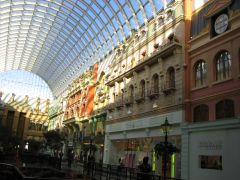
\includegraphics[width=.45\linewidth]{gfx/example_1}} \quad
\subfloat[Pan ma signo.]
{\label{fig:example-b}

\includegraphics[width=.45\linewidth]{gfx/example_2}} \\
\subfloat[Methodicamente o uno.]
{
\includegraphics[width=.45\linewidth]{gfx/example_3}} \quad
\subfloat[Titulo debitas.]
{
\includegraphics[width=.45\linewidth]{gfx/example_4}}
\caption[Tu duo titulo debitas latente]{Tu duo titulo debitas latente.}\label{fig:example}
\end{figure}